\chapter{Il flusso unidirezionale con Flux e Redux}
E' stato spiegato come MVC gestisce la problematica del flusso dei dati attraverso la bidirezionalità, e tutti i problemi che quest'ultima causa nell'implementazione di una applicazione web complessa. Solo recentemente è stato implementato un nuovo tipo di approccio che cerca di ovviare a tutto ciò, ed è quello del “flusso unidirezionale”. Due sono le architetture che verranno analizzate: Flux e Redux, entrambe riescono a mantenere un alto livello di scalabilità a prescindere dalla complessità dell'applicazione e risolvono tutti i problemi legati al flusso bidirezionale ed MVC.

\section{Architettura Flux}
\label{FluxArchitecture}
Flux è un'architettura recente creata da Facebook che struttura il front-end di una applicazione in modo che il flusso dei dati dall'innesco di un evento fino alle sue ripercussioni nell'interfaccia segua un'unica direzione.
Questo pattern, essendo molto astratto, non ha delle vere e proprie dipendenze ed è possibile applicarlo a qualsiasi tipo di applicazione con qualsivoglia linguaggio. È tuttavia nato per strutturare applicazioni React e quindi perfezionato per tale libreria.

\begin{figure}[h]
\centering
\vspace*{0.5cm} 
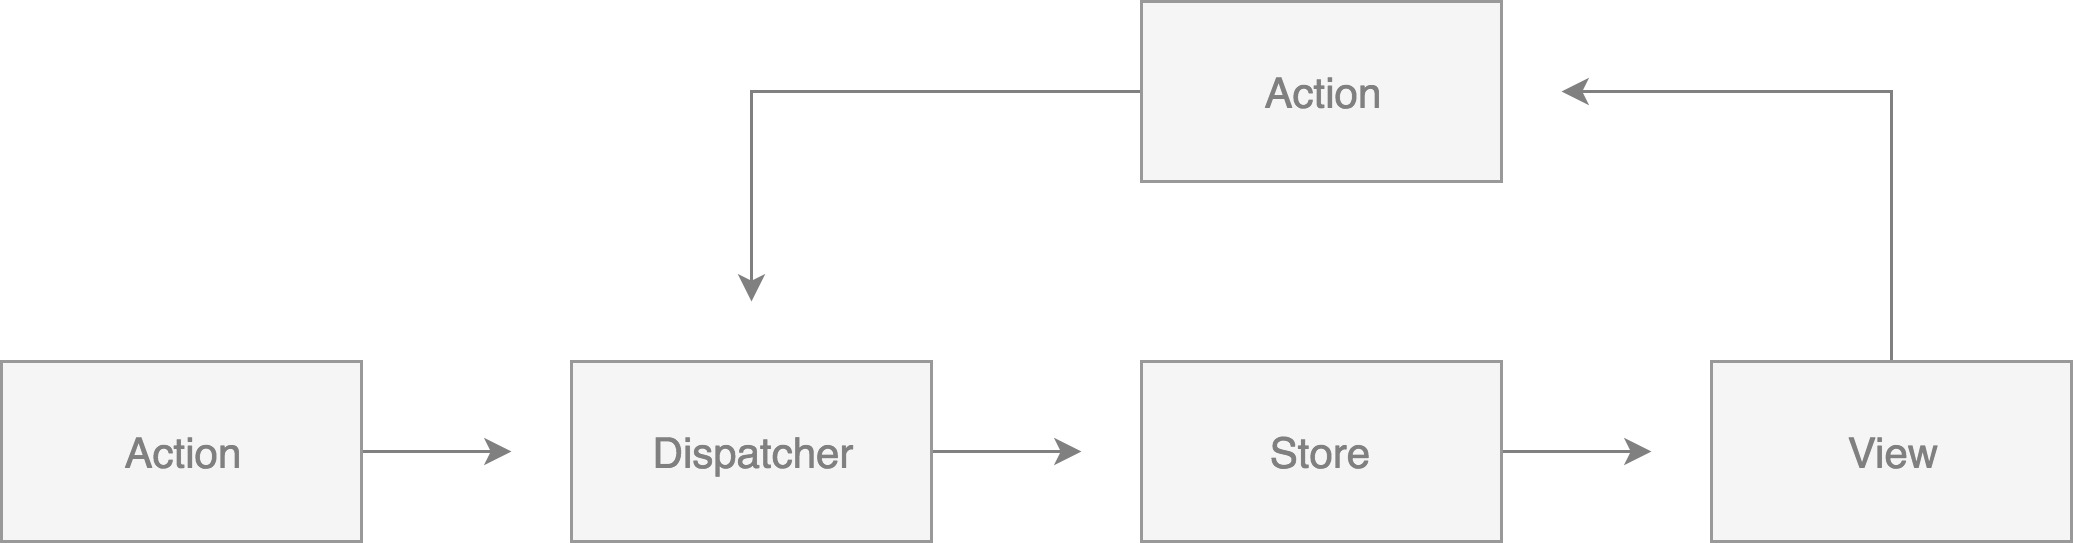
\includegraphics[width=14cm]{./images/FluxWorkflow}
\caption{Rappresentazione del flusso di dati con Flux.}
\label{FluxWorkflow}
\vspace*{0.5cm} 
\end{figure}

La struttura di questa architettura è rappresentata nella Figura \ref{FluxWorkflow}. La sua logica è divisa in due parti: ciò che riguarda gli eventi e le modifiche all'interfaccia è compreso nella View, la quale potrebbe essere definita come una Controller-View in quanto esegue entrambi i lavori; la logica che riguarda invece lo stato dell'applicazione è compresa negli Store, i quali a seconda dell'azione eseguita lo modificano di conseguenza

\subsection{I componenti}
\label{FluxComponents}
Flux considera nella sua architettura quattro elementi fondamentali: Le \textit{Action}, il \textit{Dispatcher}, gli \textit{Stores} e le \textit{View}.

\subsubsection*{Action}
Le Action sono la moneta di scambio dell'architettura e vengono propagate dalle View (attraverso il Dispatcher) agli Store che le utilizzeranno per apportare modifiche a se stessi. Queste consistono generalmente in un oggetto composto da due elementi:

    \begin{itemize}
        \item \textbf{Nome} Rappresenta lo scopo dell'azione da effettuare, ed è una stringa come ad esempio \mintinline{text}{AddArticle} o \mintinline{text}{RemoveUser}. 
        \item \textbf{Payload} È l'insieme di dati necessari a portare a termine l'azione. Se si stesse parlando di una azione \mintinline{text}{AddArticle} ad esempio, il payload sarebbe composto dal titolo e dal contenuto dell'articolo da aggiungere.
    \end{itemize}

Tutti gli eventi esistenti che modificano lo stato dell'applicazione devono essere descritti sotto forma di Action. In Flux qualsiasi cosa non sia un'azione non può verificarsi.

\subsubsection*{Dispatcher}
Il Dispatcher nell'architettura Flux è il componente che ha il compito di distribuire le Action agli Store. È sostanzialmente un registro di callback, e non ha una vera e propria logica sua fungendo quindi solo da trasmettitore. La sua particolarità è che qualsiasi azione riceva, viene trasmessa poi ad ogni callback registrata lasciando a quest'ultima il compito di analizzare l'azione e decidere se effettuare cambiamenti o meno.

\begin{listing}[ht]
\inputminted{javascript}{sources/fluxDispatcherExample.js}
\caption{Esempio di un semplice Dispatcher.} 
\label{applicationMVCPresenterEvents} 
\end{listing} 

Normalmente come Dispatcher viene utilizzato quello già implementato contenuto nella libreria Javascript \textit{Flux}\footnote{https://github.com/facebook/flux/blob/master/src/Dispatcher.js}. La particolarità di questo è che permette di gestire azioni con dipendenze, ossia azioni che dipendono dalla corretta esecuzione di altre azioni precedenti. Man mano che una applicazione cresce è molto probabile trovare dipendenze legate a Store differenti. Quando ad esempio lo “Store X" ha bisogno che lo “Store Y” si aggiorni prima effettuare i propri cambiamenti, c'è bisogno che il Dispatcher sia in grado di sincronizzare i due eventi. Ciò avviene tramite il metodo \mintinline{text}{Dispatcher.waitFor()}, che blocca l'esecuzione della callback dove viene eseguito attendendo che tutte le altre callback passate a quest'ultimo come parametro vengano completate.

\subsubsection*{Store}
Lo Store dell'architettura Flux può essere paragonato al Model del paradigma MVC. Si occupa di mantenere parte dello stato dell'applicazione, di ottenere i dati, di emettere eventi e di fornire la callback per la gestione delle Action al Dispatcher. Questa callback non è altro che una funzione che prende in input l'Action emessa dal Dispatcher e con all'interno un costrutto \mintinline{text}{Switch} che determina cosa fare. Se l'Action è stata eseguita dallo Store, questo emetterà un evento e tutte le View in ascolto di questo particolare evento si aggiorneranno di conseguenza.

\begin{figure}[h]
\centering
\vspace*{0.5cm} 
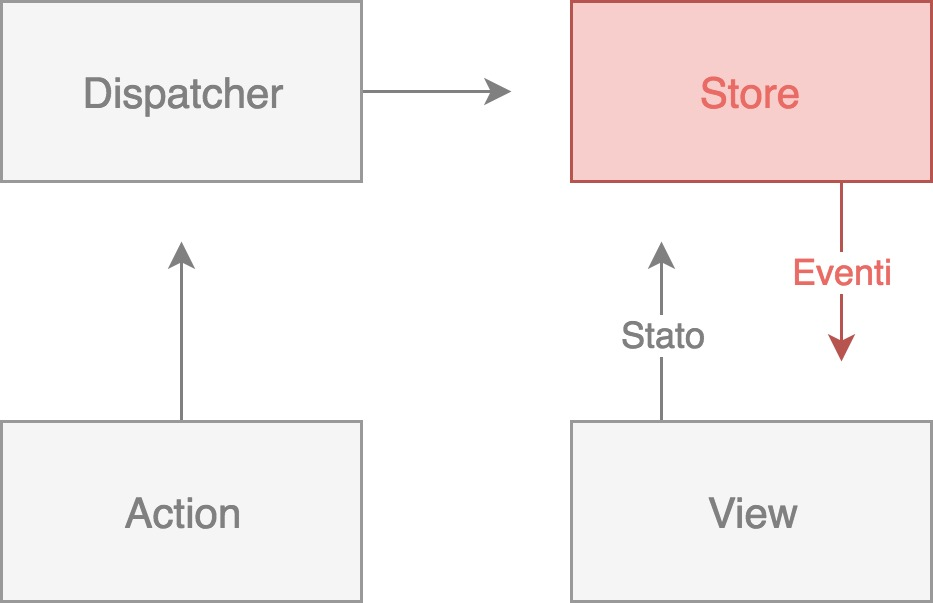
\includegraphics[width=6.5cm]{./images/StoreWorkflow}
\caption{Compiti dello Store nell'architettura Flux.}
\label{StoreWorkflow}
\vspace*{0.5cm} 
\end{figure}

Un punto fondamentale riguardo gli Stores è che essi non ricevono modifiche esterne. Tutta la logica relativa al cambiamento dello stato dell'applicazione è contenuta al loro interno e questo semplifica enormemente il lavoro di debugging del codice e rafforza la consistenza dello stato.

\subsubsection*{View}
La View è formata da componenti React strutturati presumibilmente con il pattern spiegato nella Sezione \ref{ReactExplanation}, dei componenti contenitori e di presentazione. Nel caso di Flux, i componenti contenitori sono posizionati al livello più alto ed interagiscono direttamente con gli Store, rimanendo in ascolto dei loro eventi e ottenendo da essi i dati che verranno poi passati ai componenti di presentazione figli.
Utilizzando questa strategia si assicura un corretto flusso dei dati, in cui l'unico punto di ingresso è il componente contenitore all'inizio della catena.

\subsection{Analisi dell'applicazione}
\label{FluxApplication}
Per avere un esempio pratico di questa architettura verrà implementata di nuovo l'applicazione presentata nella Sezione \ref{ExampleApplicationMVC}, questa volta attraverso React e Flux.
In questo caso oltre che la normale sintassi di ES6 c'è anche bisogno di compilare il codice JSX all'interno di questa in modo da ottenere i componenti React desiderati, per questo motivo verrà utilizzato anche il plugin di Babel \textit{React Preset}\footnote{https://babeljs.io/docs/plugins/preset-react}.
Vengono utilizzati due tipi di configurazioni per Webpack: \mintinline{text}{webpack.dev.js} in fase di development, più veloce ma che genera un codice non ottimizzato; \mintinline{text}{webpack.prod.js} in fase di produzione, più lenta che genera però un codice più leggero e veloce.

Il codice dell'applicazione è diviso in due parti principali: i componenti React nella cartella \mintinline{text}{flux/src/components} e gli elementi dell'architettura Flux nella cartella \mintinline{text}{flux/src/data}. Di seguito verranno spiegate in dettaglio queste due parti.

\subsubsection*{I componenti React}
Il componente più ad alto livello in cui viene inizializzata l'applicazione e dove React viene aggiunto materialmente al DOM è situato in \mintinline{text}{flux/src/app.js}. Salta subito all'occhio che questo è un componente “di passaggio” ed utilizzato solo per inizializzare React. Il vero e proprio componente più ad alto livello, e che possiamo considerare come componente “container” è \mintinline{text}{flux/src/components/Bookshelf.js}.

\begin{listing}[ht]
\inputminted{javascript}{sources/applicationFluxBookshelfState.js}
\caption{Esempio di interazione tra componente container e Store.} 
\label{applicationFluxBookshelfState} 
\end{listing} 

Il Codice \ref{applicationFluxBookshelfState} rappresenta l'interazione tra il componente container Bookshelf e lo Store principale dell'applicazione. Questa interazione si divide in due parti: 

\begin{enumerate}
    \item Nel costruttore viene inizializzato lo stato del componente ottenendolo dallo Store tramite il metodo \mintinline{text}{BookshelfStore.getBooks()}.

    \item Nel metodo \mintinline{text}{componentWillMount()}, che React esegue automaticamente durante l'inizializzazione del componente, viene iniziato l'ascolto dell'evento di aggiornamento dello Store assegnandolo alla funzione interna \mintinline{text}{_onChange()} che provvederà a sincronizzare lo stato del componente con quello dello Store.
\end{enumerate}

Il componente container ha poi il compito di comporre l'interfaccia utilizzando gli altri componenti di presentazione a disposizione, e passare loro i dati e le funzioni per il corretto funzionamento dell'applicazione.

\begin{listing}[ht]
\inputminted{jsx}{sources/applicationFluxBookshelfRender.js}
\caption{Esempio di composizione tra componente container e di presentazione.} 
\label{applicationFluxBookshelfRender} 
\end{listing} 

Nel Codice \ref{applicationFluxBookshelfRender} viene utilizzato il componente \mintinline{text}{<AddBook />} definito all'interno del file \mintinline{text}{AddBook.js}, al quale viene passata la funzione \mintinline{text}{_handleAddBook(title, author)} che gestirà l'evento di aggiunta di un nuovo libro emanando l'Action relativa al Dispatcher. Tutti i componenti di presentazione utilizzati per comporre l'interfaccia sono dipendenti dal componente container \mintinline{text}{<Bookshelf />} e non comunicano direttamente con l'architettura Flux. Un componente di presentazione è solitamente composto solamente da una funzione che ritorna codice JSX in base alle proprietà ricevute dal componente superiore.

\begin{listing}[ht]
\inputminted{jsx}{sources/applicationFluxButton.js}
\caption{Esempio di un semplice componente di presentazione.} 
\label{applicationFluxButton} 
\end{listing} 

Ad esempio il componente rappresentato nel Codice \ref{applicationFluxButton}, che rappresenta un semplice bottone, è riutilizzabile all'interno dell'applicazione in quanto a seconda del contesto possiamo cambiare il suo contenuto e comportamento a seconda delle proprietà passate.

E' possibile creare un componente contenitore all'interno di un altro, se è necessario gestire elementi dell'interfaccia piuttosto complessi. Questo è il caso del componente \mintinline{text}{<AddBook />}, che rappresenta il form di aggiunta di un nuovo libro, composto dai vari campi di testo ed il bottone di invio, e mantiene al suo interno lo stato di questi vari elementi. È bene prestare attenzione nell'aggiungere componenti contenitori nidificati, sopratutto nel non utilizzarli per interagire con l'architettura, compito che dovrebbe essere lasciato sempre al componente di più alto livello.

\subsubsection*{La gestione dei dati}
L'architettura Flux è implementata attraverso i componenti presenti nella cartella \mintinline{text}{flux/src/data}. Il primo file da analizzare è \mintinline{text}{BookshelfActions.js}, una libreria che fornisce le Actions eseguibili all'interno dell'applicazione sotto forma di funzione, e le fa emettere direttamente dal Dispatcher. Questo tipo di utility è comunemente chiamata in ambito Flux \textit{ActionCreator}.

\begin{listing}[ht]
\inputminted{jsx}{sources/applicationFluxActions.js}
\caption{Esempio di ActionCreator dell'applicazione.} 
\label{applicationFluxActions} 
\end{listing} 

Nell'esempio del Codice \ref{applicationFluxActions} viene riportata una funzione che automatizza l'emissione dell'azione \mintinline{text}{ADD_BOOK} al Dispatcher, fornendo come payload il titolo e l'autore del libro.
Le funzioni implementate dall'ActionCreator vengono generalmente utilizzate dal componente container per interagire in maniera corretta con lo Store.

Le Action devono essere emesse dal Dispatcher (Codice \ref{applicationFluxDispatcher}), questo nell'applicazione viene implementato nel file \mintinline{text}{BookshelfDispatcher.js} utilizzando quello messo a disposizione automaticamente dalla libreria \textit{Flux}. Questo Dispatcher, implementato ed attualmente utilizzato anche da Facebook, è una versione molto più potente del codice esempio esposto nella Sezione \ref{FluxComponents}.

\begin{listing}[ht]
\inputminted{jsx}{sources/applicationFluxDispatcher.js}
\caption{Dispatcher dell'applicazione.} 
\label{applicationFluxDispatcher} 
\end{listing} 

Viene esportata direttamente un'istanza che ci fornisce un singleton, in quanto il Dispatcher deve essere unico all'interno dell'applicazione e condiviso tra tutti i componenti che hanno bisogno di effettuare azioni.

L'ultimo componente che viene preso in esame è lo Store, implementato nel file \mintinline{text}{BookshelfStore.js}. Questo ha il compito di gestire lo stato dell'applicazione mantenendo una lista di libri in \mintinline{text}{this.state}, pre-popolata attraverso il file JSON \mintinline{text}{db.json}, e anche quello di fornire al Dispatcher la funzione incaricata di gestire le Action emesse.

\begin{listing}[ht]
\inputminted{jsx}{sources/applicationFluxStore.js}
\caption{Registrazione dello Store nel Dispatcher} 
\label{applicationFluxStore} 
\end{listing}

Analizzando il Codice \ref{applicationFluxStore} è possibile notare che lo Store viene creato estendendo la classe \mintinline{text}{EventEmitter}, questo perché ogni Store ha la necessità di mandare eventi all'interno dell'applicazione ogni qualvolta lo stato viene modificato. Troviamo poi all'interno del costruttore della classe il metodo \mintinline{text}{BookshelfDispatcher.register()} che prende come parametro la funzione dello Store da registrare nel Dispatcher. La funzione che verrà aggiunta è \mintinline{text}{_registerActions()} la quale prende come parametro un'Action e, come da prassi, la getta in pasto ad un costrutto \mintinline{text}{Switch} che la eseguirà sullo Store corrente.


\subsection{Flux e il flusso dei dati}
Come possiamo notare dalla Sezione \ref{FluxApplication}, l'architettura di Flux rispetto a quella MVC è molto più strutturata, ed i dati e gli eventi devono sottostare a delle regole e dei percorsi più rigidi, cosa che permette di avere un maggiore controllo sui comportamenti dell'applicazione e sui cambiamento dello stato. In Flux gli effetti collaterali derivati dall'aggiornamento dello stato sono molto facili da controllare, e grazie alla rigidità dell'architettura anche in numero molto inferiore. Quando uno Store riceve un'Action, ed il suo stato viene modificato, emette un evento grazie al quale le View dell'applicazione si modificheranno di conseguenza. Questo è l'unico, ed inevitabile, caso in cui la modifica dello stato causa un'ulteriore esecuzione di codice. 
Tuttavia il vantaggio di Flux non sta solo in questo, ma anche nel gestire in modo chiaro le dipendenze tra due Store differenti. In un'architettura MV* non esiste un vero e proprio approccio che permette di eseguire un cambiamento solo se ne è stato fatto un'altro in precedenza, se non in maniera imperativa e notificando manualmente il componente dipendente. In Flux questo problema è risolto semplicemente dichiarando la dipendenza all'interno dello Store tramite la funzione \mintinline{text}{Dispatcher.waitFor()} descritta nella Sezione \ref{FluxComponents}.
Un altro elemento a favore di Flux riguarda sempre lo Store e come questo integri in se stesso tutti i possibili cambiamenti che lo stato possa fare. Ciò fa sì che nel caso in cui si debba analizzare un certo cambiamento, la sua posizione all'interno del codice sia immediata. Questo impedisce la creazione di cambi di stato nascosti o non previsti, classici durante lo sviluppo di applicazioni MV* \cite{boduch2016flux}.

Tutto ciò espresso fino ad ora è indubbiamente un punto a favore a livello di architettura, di gestione dei dati e degli eventi, tuttavia a livello implementativo possono sorgere dei difetti non trascurabili.
In Flux lo Store notifica le View del cambiamento del proprio stato, senza specificare cosa è stato cambiato come ad esempio potrebbe capitare in altre architetture. Questo comporta un lavoro più oneroso da parte della View, la quale potrebbe dover aggiornare, anche inutilmente, più componenti del necessario. Proprio per questo motivo React è considerato un'ottima libreria per Flux in quanto riesce ad aggiornare solamente il DOM che viene effettivamente modificato.
Un'altra problematica sempre riguardo gli Store è quando il loro numero e la loro complessità diventa elevata, e di conseguenza diventa molto difficile gestire le dipendenze delle Action nonostante la presenza del Dispatcher. Queste dipendenze possono diventare sempre più numerose, complesse e difficili da gestire all'aumentare del numero di features dell'applicazione.
Un altro punto a sfavore di Flux riguarda le Action. Ogni cosa che accade all'interno dell'applicazione deve essere descritta con un'Action, ed facile immaginare che una singola feature può dunque crearne un numero non irrilevante. Tenere traccia di ognuna di esse diventa quindi un compito non proprio semplice nonostante l'aiuto di una libreria ActionCreator.

\section{Architettura Redux}
\label{ReduxArchitecture}

Redux è una libreria scritta da Dan Abramov e Andrew Clark per la gestione dello stato in applicazioni web scritte con Javascript. Evolve l'idea dell'architettura Flux spiegata nella Sezione \ref{FluxArchitecture} semplificandola attraverso pattern e tecniche della programmazione funzionale. Il concetto base di Redux è che lo stato completo di una applicazione dovrebbe essere descritto attraverso un solo e semplice oggetto Javascript.

\begin{listing}[ht]
\inputminted{javascript}{sources/exampleReduxState.js}
\caption{Stato di una applicazione scritta con Redux preso dal sito ufficiale.} 
\label{exampleReduxState} 
\end{listing}

Nel Codice \ref{exampleReduxState} preso dal sito ufficiale di Redux ad esempio, viene rappresentato lo stato completo di una applicazione per la gestione delle cose da fare (la classica “To-do application”), con anche dei filtri per visualizzare i compiti aggiunti.

\begin{figure}[h]
\centering
\vspace*{0.5cm} 
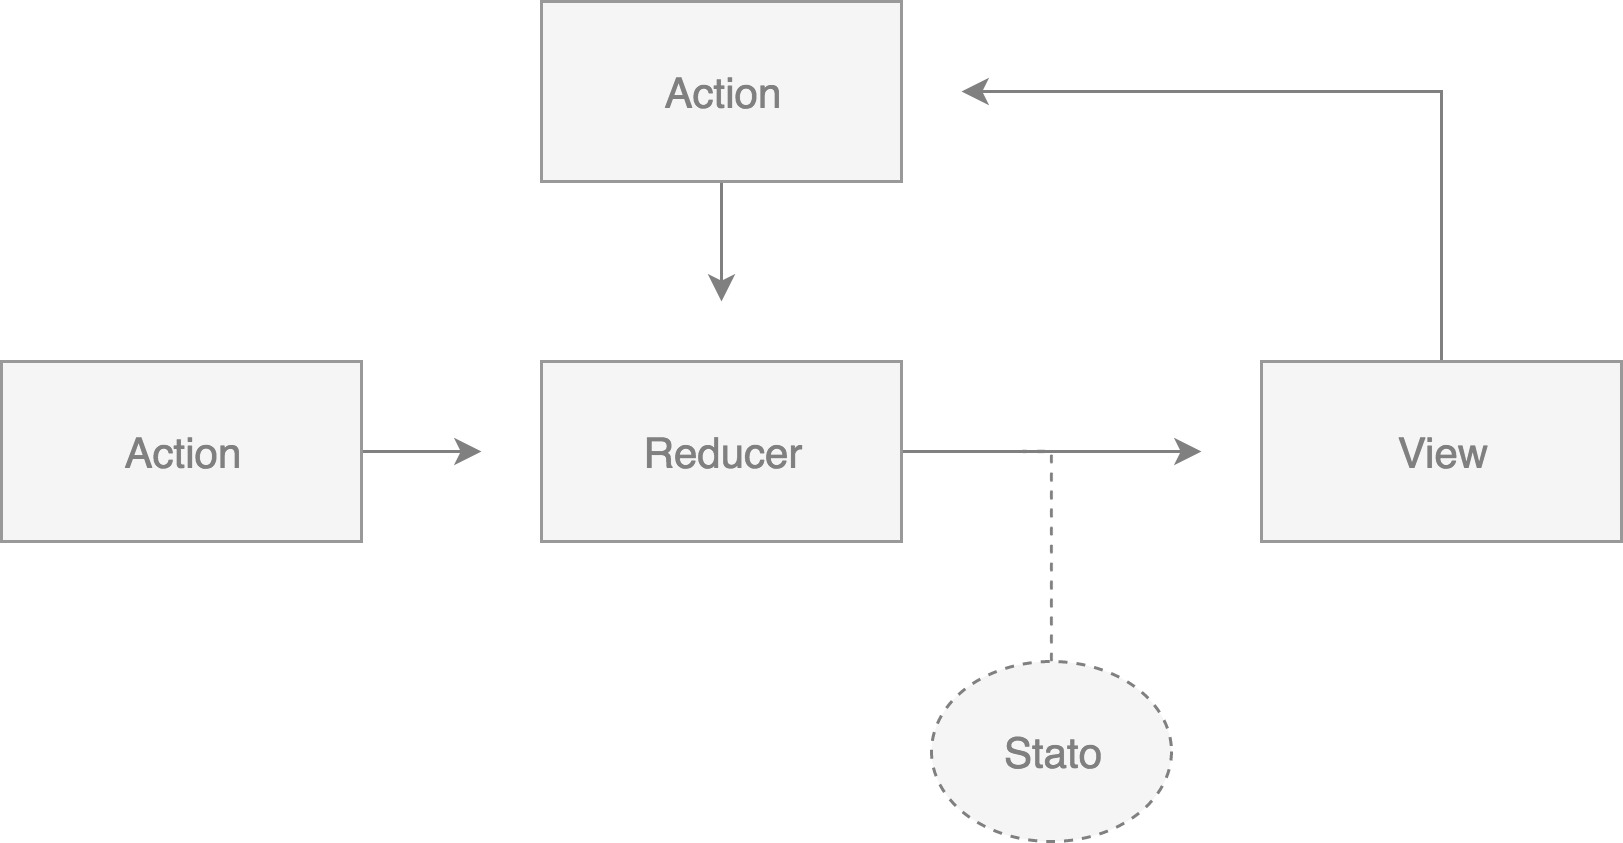
\includegraphics[width=11.5cm]{./images/ReduxWorkflow}
\caption{Architettura Redux}
\label{ReduxWorkflow}
\vspace*{0.5cm} 
\end{figure}

Come è possibile notare nella Figura \ref{ReduxWorkflow}, Redux è molto simile a Flux, ereditando cose come la completa gestione logica dello stato all'interno di un singolo componente, che in Flux era lo Store ma che in Redux è il \textit{Reducer}. Un altro elemento in comune riguarda l'uso delle \textit{Action}, le quali andando in input a al Reducer permettono di modificare lo stato all'interno dello Store. Il Reducer quindi non è altro che una funzione che prende in input lo stato attuale ed una Action, restituendo in output il nuovo stato da loro derivato.
Al contrario di Flux tuttavia non esiste un Dispatcher in quanto i Reducers sono \textit{funzioni pure}\footnote{Una funzione pura è una funzione che, dati gli stessi input, restituisce lo stesso output e non ha nessun effetto collaterale, come ad esempio richieste al database, o mutazioni a variabili fuori dal suo scope \cite{FranklinOnPureFunctions}.}, facili da comporre e che non hanno quindi bisogno di un componente esterno che li gestisca. Questa può essere vista sia come una differenza di implementazione che come un miglioramento, in quanto la gestione dello stato di Flux è stata sempre descritta come una funzione che deriva il nuovo stato dal precedente e dall'azione eseguita su di esso \mintinline{text}{(state, action) => state}, descrivendo precisamente quello che è il Reducer in Redux \cite{ReduxDocumentation}.

\subsection{I tre principi base di Redux}
Per scrivere una applicazione che segue in modo preciso questa architettura è necessario seguire tre principi basilari che ne accertano il giusto utilizzo \cite{ReduxDocumentation}:

\begin{enumerate}
    \item \textbf{Una sola fonte di verità} Il primo principio indica che lo stato di una applicazione deve essere unico e deve essere memorizzato all'interno di un singolo Store.
    Questo facilita operazioni come la serializzazione dello stato attuale in modo da poterlo salvare, ad esempio in un database, e recuperarlo in seguito per ripristinare l'applicazione ad un momento precedente. Oppure implementare funzionalità che normalmente sarebbero piuttosto complicate, come l'azione di annullare un'operazione effettuata.
    Avere a disposizione uno stato singolo per applicazione semplifica anche le operazioni di debugging e di ispezione.

    \item \textbf{Lo stato in sola lettura} Il secondo principio di Redux, e comune anche a Flux, dice che lo stato dell'applicazione non può essere modificato se non per mezzo dell'emissione di un'Action al Reducer. Questo assicura che nessun componente possa inavvertitamente apportare modifiche dirette allo stato e generare quindi comportamenti inaspettati ed imprevedibili.

    \item \textbf{Lo stato cambia solo attraverso funzioni pure} Il terzo ed ultimo principio, ma non a livello di importanza, riguarda l'obbligo di utilizzare solamente funzioni pure all'interno dei Reducer. Questo permette di comporre più Reducer specifici nell'unico Reducer che si occupa della gestione dello stato, e siccome questi sono solamente funzioni senza effetti collaterali è possibile controllare il loro ordine di esecuzione o creare Reducer generici per parti dello stato comuni.
\end{enumerate}

\subsection{I componenti}
Due sono i cambiamenti fondamentali dei componenti di Redux rispetto a quelli di Flux descritti nella Sezione \ref{FluxComponents}: il primo consiste nell'abbandono del Dispatcher; il secondo riguarda invece lo Store che questa volta è unico all'interno dell'applicazione e sfrutta la funzione Reducer per la gestione logica dello stato.

\subsubsection*{Action}
Anche in Redux come nell'architettura Flux le Action sono semplici oggetti composti da un “nome” e da un “payload”, e anche qui si utilizza una libreria ActionCreator per una loro gestione più facile e comprensibile. La differenza principale tuttavia è che in Flux l'ActionCreator eseguiva direttamente \mintinline{text}{Dispatcher.dispatch()} ed emettendo quindi direttamente l'Action, in Redux invece l'ActionCreator si occupa solamente di restituire l'oggetto Action desiderato. Astrarre l'Action in questo modo è utile perché la funzione \mintinline{text}{dispatch()} che si occupa di emettere l'azione al Reducer è possibile ottenerla sia dallo Store con \mintinline{text}{Store.dispatch()} sia dalla funzione \mintinline{text}{connect()} presente nella libreria \textit{react-redux}\footnote{https://github.com/reactjs/react-redux} che automatizza la creazione del componente container in React e gestisce tutti i suoi aggiornamenti in maniera molto più efficiente che facendolo a mano sottoscrivendolo allo Store.

\subsubsection*{Reducer}
Il Reducer è il cuore dell'architettura Redux, nonché il componente che racchiude tutto il significato di quest'ultima ed il perché della sua potenza. Questo, come è stato precedentemente detto, è una funzione pura del tipo \mintinline{text}{(state, action) => state}, ossia che prende come parametro lo stato attuale dell'applicazione ed una Action, restituendo il nuovo stato. Il Reducer è comparabile in Flux alla funzione che dallo Store registriamo nel Dispatcher per gestire un'Action.
Siccome lo stato, in questa architettura, è unico (deve essere rappresentato in un singolo oggetto Javascript) come è unico anche lo Store, e quindi anche la funzione Reducer, è necessario trovare un modo per organizzare quest'ultima in maniera comprensibile. Se si dovesse scrivere il Reducer per esteso si otterrebbe una funzione lunghissima e difficilmente gestibile anche per una applicazione non troppo grande, tuttavia utilizzando il pattern della composizione presente nella programmazione funzionale è possibile ovviare a questo problema in modo molto semplice.

\begin{listing}[ht]
\inputminted{javascript}{sources/exampleReduxReducer.js}
\caption{Esempio di composizione fra Reducer.} 
\label{exampleReduxReducer} 
\end{listing}

Come rappresentato nel Codice \ref{exampleReduxReducer} è possibile creare un Reducer isolato per ogni elemento dello stato da gestire, e comporli insieme per formare il Reducer principale attraverso la funzione \mintinline{text}{combineReducers()} messa a disposizione dalla libreria Redux. Questa funzione non fa altro che chiamare i Reducer creati con il pezzo di stato a loro assegnato, combinando tutti i risultati ottenuti in un singolo oggetto \cite{ReduxDocumentation}.

\subsubsection*{Store}
Lo Store nell'architettura Redux rappresenta il componente che integra sia il Reducer che le Action. Lo Store è incaricato di tenere traccia dello stato dell'applicazione, fornire lo informazioni sullo stato ai componenti della View, aggiornare lo stato attraverso la funzione \mintinline{text}{dispatch()} e sottoscrivere i componenti interessati all'aggiornamento dello stato in modo che siano notificati.
Una volta creato il Reducer principale dell'applicazione, la costruzione dello Store è praticamente immediata utilizzando la funzione \mintinline{text}{createStore()} che prende come primo parametro il Reducer, e come secondo parametro opzionale uno stato iniziale.

\subsubsection*{View}
La View di Redux, usando React, è quasi del tutto simile ad una View dell'architettura Flux, con qualche differenza riguardo ai componenti container. Per interagire con l'architettura Redux dal componente container è possibile utilizzare due metodi diversi, uno manuale ed un altro automatizzato:

\begin{itemize}
    \item \textbf{Metodo manuale} In questo caso la comunicazione con l'architettura Redux avviene attraverso la sottoscrizione del componente container allo Store attraverso la funzione \mintinline{text}{Store.subscribe()} in modo da poterne ottenere lo stato, e la gestione sempre manuale delle proprietà di tutti i componenti di presentazione collegati. Questo metodo è quello adottato anche nell'architettura Flux.

    \item \textbf{Metodo automatizzato} La libreria Redux mette a disposizione la funzione \mintinline{text}{connect()} che permette di creare in maniera automatica il componente contenitore. Questa riceve in input due funzioni chiamate: \mintinline{text}{mapStateToProps()} e \mintinline{text}{mapDispatchToProps()}. La prima permette di tradurre lo stato ottenuto dallo Store nelle proprietà da passare poi ai vari componenti di presentazione collegati. La seconda permette invece di definire i metodi che eseguono la funzione \mintinline{text}{dispatch()} per l'emissione delle Action.
\end{itemize}

Utilizzare la funzione \mintinline{text}{connect()} per la generazione del componente contenitore è estremamente preferibile in quanto apporta delle ottimizzazioni automatiche (come l'implementazione della funzione interna \mintinline{text}{shouldComponentUpdate()}\footnote{La funzione \textit{shouldComponentUpdate} permette di modificare il sistema di aggiornamento del componente React dove essa è definita. Di default un componente si aggiorna ogni volta che le sue proprietà vengono modificate, e quindi la funzione ritorna sempre \textit{true}. Se non vogliamo aggiornare un componente, o vogliamo che il suo aggiornamento avvenga solo in casi particolari è necessario modificare \textit{shouldComponentUpdate} affinché ritorni \textit{false} quando necessario.} dei componenti React) per evitare di far effettuare aggiornamenti inutili ai componenti, ad ogni modifica dello stato nello Store.

Tutti i componenti container potrebbero aver bisogno di accedere allo Store, in qualsiasi posizione dell'applicazione essi siano, specialmente se la comunicazione con l'architettura avviene in maniera manuale. Un'opzione è quella di passarlo come proprietà ad ogni livello gerarchico della View, tuttavia potrebbe risultare un'azione ripetitiva e piuttosto tediosa specialmente se abbiamo dei componenti container nidificati. Un'altra utile feature di Redux riguarda il componente \mintinline{text}{<Provider />}. Utilizzandolo solo una volta ed al livello più alto dell'applicazione rende lo Store disponibile ad ogni componente senza doverlo passare esplicitamente \cite{ReduxDocumentation}.

\subsection{Analisi dell'applicazione}
Per l'analisi concreta di un'applicazione con Redux, verrà ripreso parte del codice dell'architettura Flux implementato nella Sezione \ref{FluxApplication}. Le dipendenze sono sempre le stesse ad eccezione delle librerie dell'architettura, ed in questo caso dell'aggiunta di \textit{react-redux}. Come le stesse sono anche le due configurazioni di Webpack.

Il codice è sempre diviso in due parti principali: i componenti React nella cartella \mintinline{text}{redux/src/components} e gli elementi dell'architettura Redux in questo caso, nella cartella \mintinline{text}{redux/src/data}. Di seguito verranno spiegate in dettaglio queste due parti e le principali differenze con l'architettura Flux.

\subsubsection*{I componenti React}
Come è già stato detto in precedenza, l'unico componente React che cambia nell'architettura Redux è il componente container, il quale non è più gestito manualmente ma automatizzato attraverso la funzione \mintinline{text}{connect()} di Redux.

\begin{listing}[ht]
\inputminted{javascript}{sources/applicationReduxBookshelf.js}
\caption{Componente container con Redux.} 
\label{applicationReduxBookshelf} 
\end{listing}

Nel Codice \ref{applicationReduxBookshelf} è rappresentato il componente container principale dell'applicazione, e come le funzioni \mintinline{text}{mapStateToProps()} e \mintinline{text}{mapDispatchToProps()} vengono connesse insieme al componente \mintinline{text}{<Bookshelf />} impacchettandolo per fornirgli tutte le informazioni necessarie dello Store attraverso le sue proprietà.

\begin{listing}[ht]
\inputminted{javascript}{sources/applicationReduxBookshelfProps.js}
\caption{Funzioni di gestione del componente container con Redux.} 
\label{applicationReduxBookshelfProps} 
\end{listing} 

Il contenuto di queste funzioni utilizzate all'interno di \mintinline{text}{connect()} è presente nel Codice \ref{applicationReduxBookshelfProps}. La funzione \mintinline{text}{mapStateToProps()} prende in input lo stato dallo Store (il quale in questa applicazione è solamente un array di libri) e lo assegna ad una proprietà. Questo procedimento è l'equivalente di assegnare lo stato dello Store in maniera diretta: \mintinline{text}{<Bookshelf books={state.books} />}.
Allo stesso modo, la funzione \mintinline{text}{mapDispatchToProps()} prende come parametro la funzione per l'emissione delle Action \mintinline{text}{dispatch()} e la assegna, utilizzando le funzioni create all'interno dell'ActionCreator, alle proprietà che serviranno per gestire gli eventi nei vari componenti di presentazione.
La funzione \mintinline{text}{connect()} prende in input queste due funzioni e restituisce in output una nuova funzione \textit{Higher-order component}\footnote{Un \textit{Higher-order component}, o più semplicemente “HOC”, è una funzione che prende in input e restituisce in output un componente React. Il suo nome deriva dalle “higher order function” che in matematica rappresentano funzioni che prendono come parametro una o più funzioni, e ritornano una o più nuove funzioni derivate da queste.}, che passa ad un componente React tutte le proprietà precedentemente definite. In questo caso il componente React passato come parametro, come è possibile notare nel Codice \ref{applicationReduxBookshelf}, corrisponde alla funzione \mintinline{text}{render()} del componente \mintinline{text}{<Bookshelf />} implementato nell'architettura Flux.

\subsubsection*{La gestione dei dati}
La vera e propria architettura Redux è implementata nei file contenuti in \mintinline{text}{redux/src/data} dove si trovano Reducer e Action, e nel file \mintinline{text}{redux/src/app.js} dove viene creato lo Store. Tecnicamente, in Redux abbiamo un solo componente che esiste concretamente, ed è lo Store. I Reducer e le Action (più precisamente l'ActionCreator in questa applicazione) servono a far funzionare nel modo corretto quest'ultimo. I primi gestiscono lo stato, le seconde permettono ai vari componenti di interagire con lo Store.
Sotto questo punto di vista Redux semplifica parecchio l'architettura di Flux, concentrando tutto il lavoro in un unico componente invece di avere un numero indefinito di Store coordinati tramite il Dispatcher.

\begin{listing}[ht]
\inputminted{javascript}{sources/applicationReduxActions.js}
\caption{ActionCreator dell'applicazione Redux.} 
\label{applicationReduxActions} 
\end{listing}

Nel Codice \ref{applicationReduxActions} è rappresentato l'ActionCreator che ritorna le varie Action da eseguire per mezzo della funzione \mintinline{text}{dispatch()}. Al contrario che nell'architettura Flux ogni funzione definita nell'ActionCreator ritorna un normale oggetto, invece che emettere direttamente l'azione allo Store.

\begin{listing}[ht]
\inputminted{javascript}{sources/applicationReduxReducer.js}
\caption{Reducer dell'applicazione Redux.} 
\label{applicationReduxReducer} 
\end{listing}

Il Reducer descritto nel Codice \ref{applicationReduxReducer} descrive il cambiamento dello stato nello Store alla ricezione di determinate Action. La struttura della funzione del Reducer è molto simile a quella della funzione registrata all'interno del Dispatcher nell'architettura Flux, tuttavia il Reducer è una funzione pura. Lo stato non viene quindi mai modificato direttamente ma viene ritornato un nuovo stato a seconda dell'Action e dello stato precedente.
Ad ogni caso dello \mintinline{text}{Switch} lo stato non viene mai modificato, bensì viene duplicato tramite \mintinline{text}{Object.assign()} modificando solamente le parti dovute.
Utilizzare il costrutto \mintinline{text}{Switch} non è obbligatorio, ma è diventato in ogni caso lo standard di Redux riguardo il componente Reducer. 

\begin{listing}[ht]
\inputminted{javascript}{sources/applicationReduxStore.js}
\caption{Store dell'applicazione Redux.} 
\label{applicationReduxStore} 
\end{listing}

Nel Codice \ref{applicationReduxStore} è raffigurato il contenuto del file \mintinline{text}{app.js}, nel quale viene creato l'unico Store dell'applicazione. Questo viene creato attraverso
la funzione \mintinline{text}{createStore} la quale prende in input il Reducer e lo stato iniziale (il quale è rappresentato dalla lista di libri nel file JSON \mintinline{text}{db.json}) e restituisce in output uno Store che tiene traccia dello stato completo dell'applicazione.
Lo Store non è posizionato in un file a parte, e non è un singleton questa vota, bensì viene passato all'interno dell'applicazione attraverso il componente \mintinline{text}{<Provider />} che permette il suo accesso a qualsiasi livello della gerarchia della View.

\subsection{Redux e il flusso dei dati}
Il flusso dei dati nell'architettura Redux può essere riassunto semplicemente in un'Action emanata dalla View che viene data in pasto al Reducer nello Store, per generare il nuovo stato dell'applicazione.
Come architettura Redux è decisamente meno complesso di Flux riuscendo a semplificare il lavoro degli Store e ad eliminare il Dispatcher. I vantaggi che offre sono comunque gli stessi, infatti la gestione del flusso unidirezionale è comunque perfetta, in aggiunta l'immutabilità del Reducer e lo stato in un singolo Store sono concetti che possono essere utili per risolvere problemi comuni tipicamente complessi.

React, come descritto nella Sezione \ref{ReactServerSideRendering}, è una libreria isomorfica che è possibile utilizzare anche lato server per implementare il server-side rendering ed ottenere quindi prestazioni maggiori integrando dati iniziali ottenuti dal server già dalla prima visualizzazione dell'interfaccia, senza dover effettuare richieste aggiuntive. Con Flux tuttavia sincronizzare lo stato iniziale con il server non è semplice, in quanto lo stato è suddiviso in Store multipli ed ognuno di essi è un singleton. Redux è nativamente più efficiente sotto questo aspetto in quanto lo stato è unico e rappresentabile come un oggetto Javascript, e la sincronizzazione con il server risulta quindi immediata senza la necessità di utilizzare API esterne.

Un altro aspetto positivo di Redux è come sia possibile implementare in maniera semplice features che si basano sulla composizione dei Reducer. Per riutilizzare funzionalità su più Reducer ad esempio non è necessario utilizzare l'ereditarietà, ma basta creare un \textit{Reducer Factory}\footnote{Un \textit{Reducer Factory} consiste in una funzione scritta secondo il design pattern \textit{Factory}, ossia una funzione che ritorna un Reducer strutturato a seconda dei parametri che le passiamo in input.} che genera altri Reducer a seconda delle esigenze.
Sempre grazie a questa tecnica sono nate librerie come ad esempio \textit{redux-undo}\footnote{https://github.com/omnidan/redux-undo}, la quale permette di implementare in maniera estremamente facile una feature complessa come quella del “undo/redo”, che permette di tenere traccia del passato dello stato, e recuperarlo se necessario \cite{AbramovOnReduxVsFlux}.

A livello di performance Redux soffre, forse in maniera peggiore, degli stessi problemi di Flux, specialmente al livello di rendering della View in quanto ad ogni azione l'intero stato viene aggiornato. Tuttavia tra le ottimizzazioni messe a disposizione da React, le ottimizzazioni di Redux sui componenti container (tramite la funzione \mintinline{text}{connect()}), e altre librerie come ad esempio \textit{Reselect}\footnote{https://github.com/reactjs/reselect}, che ricalcola gli elementi dello stato solo quando sono effettivamente modificati, questo problema è quasi trascurabile.